36. $y=\cfrac{x^2-x-20}{x-5}=\cfrac{(x-5)(x+4)}{x-5}=x+4,\ x
eq5.$
$$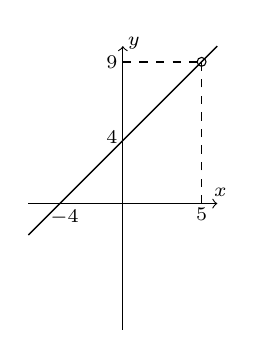
\begin{tikzpicture}[scale=0.2]
\tikzset {line01/.style={line width =0.5pt}}
\tikzset{line02/.style={line width =1pt}}
\tikzset{line03/.style={dashed,line width =0.5pt}}
%\filldraw [black] (0,0) circle (1pt);
\draw [->] (-6,0) -- (6,0);
\draw [->] (0,-8) -- (0,10);
\draw[line01] (-6,-2) -- (6,10);
\draw[line03] (5,0) -- (5,9);
\draw[line03] (0,9) -- (5,9);
%\draw[line03] (0,-2) -- (1,-2);
\draw (6.2,0.7) node {\scriptsize $x$};
%\draw (-1.2,-2) node {\scriptsize $-2$};
%\draw (-0.7,2) node {\scriptsize $2$};
\draw (-0.7,4.2) node {\scriptsize $4$};
\draw (-0.7,9) node {\scriptsize $9$};
\draw (5,-0.7) node {\scriptsize $5$};
\draw (-3.7,-0.9) node {\scriptsize $-4$};
\draw (0.7,10.2) node {\scriptsize $y$};
%\draw (1,0) circle (8pt);
\draw (5,9) circle (8pt);
\end{tikzpicture}$$
